\documentclass{article}
\usepackage[utf8]{inputenc}
\usepackage{geometry}
\usepackage{graphicx}
\usepackage{wrapfig}
\usepackage{subfig}
\usepackage{subfigure}
\usepackage{amsmath}
\usepackage{amsfonts}
\usepackage{amsthm}
\usepackage[most]{tcolorbox}
\usepackage{fancybox}
\usepackage{verbatim}
\usepackage{array}
\usepackage{latexsym}
\usepackage{alltt}
\usepackage{hyperref}
\usepackage{textcomp}
\usepackage{color}
\usepackage{float}
\usepackage{pdfpages}
\usepackage{algorithm}
\usepackage[noend]{algpseudocode}
\usepackage{multicol}


\geometry
{
 a4paper,
 left=15mm,
 top=15mm,
}

\newtcolorbox{mybox}[3][]
{
  colframe = #2!25,
  colback  = #2!10,
  coltitle = #2!20!black,  
  title    = {#3},
  #1,
}

\renewcommand\qedsymbol{$\triangle$}

\newenvironment{example}{\begin{mybox}{green}{\textbf{Example}}}{\end{mybox}}
\newenvironment{definition}[1]{\begin{mybox}{blue}{\textbf{Definition #1}}}{\end{mybox}}
\newenvironment{theorem}[1]{\begin{mybox}{red}{\textbf{Theorem #1}}}{\end{mybox}}

\title{CENG 242 - Chapter 1: Introduction}
\author{Burak Metehan Tunçel}
\date{March 2022}

\begin{document}

\maketitle

\section{Programming Linguistics}

We sometimes use the term \textbf{programming linguistics} to mean \textit{the study of programming languages}. This is by analogy with the older discipline of \textit{linguistics}, which is the study of natural languages. Both programming languages and natural languages have \textit{\textbf{syntax}} (form) and \textit{\textbf{semantics}} (meaning). However, we cannot take the analogy too far. Natural languages are far broader, more expressive, and subtler than programming languages. 

A natural language is just what a human population speaks and writes, so linguists are restricted to analyzing existing (and dead) natural languages. On the other hand, programming linguists can not only analyze existing programming languages; they can also design and specify new programming languages, and they can implement these languages on computers.

Programming linguistics therefore has several aspects.

\subsection{Concepts and Paradigms}

Every programming language is an artifact, and as such has been consciously
designed. Some programming languages have been designed by a single person
(such as C++), others by small groups (such as C and JAVA), and still others by large groups (such as ADA). A programming language, to be worthy of the name, \textit{must satisfy certain fundamental requirements}.

A programming language must be \textbf{universal}. That is to say, every problem must have a solution that can be programmed in the language, if that problem can be solved at all by a computer. This might seem to be a very strong requirement, but even a very small programming language can meet it.  
Any language in which we can define recursive functions is universal. On the other hand, a language with neither recursion nor iteration cannot be universal. Certain application languages are not universal, but we do not generally classify them as programming languages.

A programming language should also be \textit{reasonably} \textbf{natural} for solving problems, at least \textit{problems within its intended application area}. For example, a programming language whose only data types are numbers and arrays might be natural for solving numerical problems, but would be less natural for solving problems in commerce or artificial intelligence. Conversely, a programming language whose only data types are strings and lists would be an unnatural choice for solving numerical problems.

A programming language must also be \textbf{implementable} on a computer. That is to say, it \textit{must be possible to execute every well-formed program in the language}. \textit{Mathematical notation (in its full generality) is not implementable}, because in this notation it is possible to formulate problems that cannot be solved by any computer. \textit{Natural languages also are not implementable}, because they are imprecise and ambiguous. Therefore, mathematical notation and natural languages, for entirely different reasons, cannot be classified as programming languages.

In practice, a programming language should be capable of an \textit{acceptably} \textbf{efficient}\textit{ implementation}. There is plenty of room for debate over what is acceptably efficient, especially as the efficiency of a programming language implementation is strongly influenced by the computer architecture. \texttt{FORTRAN, C}, and \texttt{PASCAL} programmers might expect their programs to be almost as efficient (within a factor of 2–4) as the corresponding assembly-language programs. \texttt{PROLOG} programmers have to accept an order of magnitude lower efficiency, but would justify this on the grounds that the language is far more natural within its own application area; besides, they hope that new computer architectures will eventually appear that are more suited for executing PROLOG programs than conventional architectures.

The \textbf{concepts} that underlie the design of programming languages will be studied: \textit{data} and \textit{types, variables} and \textit{storage}, \textit{bindings} and \textit{scope, procedural abstraction, data abstraction, generic abstraction, type systems, control}, and \textit{concurrency}. Although few of us will ever design a programming language, as programmers we can all benefit by studying these concepts. Whenever we have to learn a new programming language and discover \textit{how it can be effectively exploited to construct reliable and maintainable programs}, and \textit{whenever we have to decide which programming language is most suitable for solving a given problem}, we find that a good understanding of programming language concepts is indispensable. We can master a new programming language most effectively if we understand the underlying concepts that it shares with other programming languages.

Just as important as the individual concepts are the ways in which they may be put together to design complete programming languages. Different selections of key concepts support radically different styles of programming, which are called \textbf{paradigms}. There are six major paradigms.
\begin{itemize}
    \item \textit{\textbf{Imperative Programming}} is characterized by the use of variables, commands, and procedures;
    \item \textit{\textbf{Object-Oriented Programming}} by the use of objects, classes, and inheritance;
    \item \textit{\textbf{Concurrent Programming}} by the use of concurrent processes, and various control abstractions;
    \item \textit{\textbf{Functional Programming}} by the use of functions; \item \textit{\textbf{Logic Programming}} by the use of relations;
    \item \textit{\textbf{Scripting Languages}} by the presence of very high-level features. 
\end{itemize}

\subsection{Syntax, Semantics, and Pragmatics}

Every programming language has \textit{syntax}, \textit{semantics}, and \textit{pragmatics}. We have seen that natural languages also have syntax and semantics, but \textit{pragmatics is unique to programming languages}.
\begin{itemize}
    \item A programming language’s \textbf{\textit{syntax}} is concerned with the \textit{form} of programs: how expressions, commands, declarations, and other constructs must be arranged to make a well-formed program.
    \item A programming language’s \textbf{\textit{semantics}} is concerned with the \textit{meaning} of programs: how a well-formed program may be expected to behave when executed on a computer.
    \item A programming language’s \textbf{\textit{pragmatics}} is concerned with the way in which the language is intended to be used in practice.
\end{itemize}

\textbf{Syntax} influences how programs are written by the programmer, \textit{read} by other programmers, and \textit{parsed} by the computer. \textbf{Semantics} determines how programs are \textit{composed} by the programmer, \textit{understood} by other programmers, and \textit{interpreted} by the computer. \textbf{Pragmatics} influences how programmers are expected to \textit{design} and \textit{implement} programs in practice. Syntax is important, but semantics and pragmatics are more important still.

To underline this point, consider how an expert programmer thinks, given a
programming problem to solve. Firstly, \textit{the programmer decomposes the problem, identifying suitable program units} (procedures, packages, abstract types, or classes). Secondly, \textit{the programmer conceives a suitable implementation of each program unit, deploying language concepts} such as types, control structures, exceptions, and so on. Lastly, \textit{the programmer codes each program unit}. Only at this last stage does the programming language’s syntax become relevant.

Semantic and pragmatic issues will be paid most attention. A given construct might be provided in several programming languages, with variations in syntax that are essentially superficial. \textit{Semantic issues are more important}. We need to appreciate subtle differences in meaning between apparently similar constructs. We need to see whether a given programming language confuses distinct concepts, or supports an important concept inadequately, or fails to support it at all.

In order to avoid distracting syntactic variations, wherever possible we shall illustrate each concept using the following programming languages: \texttt{C, C++, JAVA}, and \texttt{ADA}. 
\begin{itemize}
    \item \texttt{C} is now middle-aged, and its design defects are numerous; however, it is very widely known and used, and even its defects are instructive. 
    \item \texttt{C++} and \texttt{JAVA} are modern and popular object-oriented languages. 
    \item \texttt{ADA} is a programming language that supports imperative, object-oriented, and concurrent programming. 
\end{itemize}
None of these programming languages is by any means perfect. The ideal programming language has not yet been designed, and is never likely to be!

\subsection{Language Processors}

\textit{Any system for processing programs – executing programs, or preparing them for execution –} is called a \textbf{language processor}. Language processors include \textit{compilers}, \textit{interpreters}, and auxiliary tools like \textit{source-code editors} and \textit{debuggers}.

\section{Historical Development}

Today’s programming languages are the product of developments that started in the 1950s. Numerous concepts have been invented, tested, and improved by being incorporated in successive programming languages. With very few exceptions, the design of each programming language has been strongly influenced by experience with earlier languages.

\begin{figure}[h!]
    \centering
    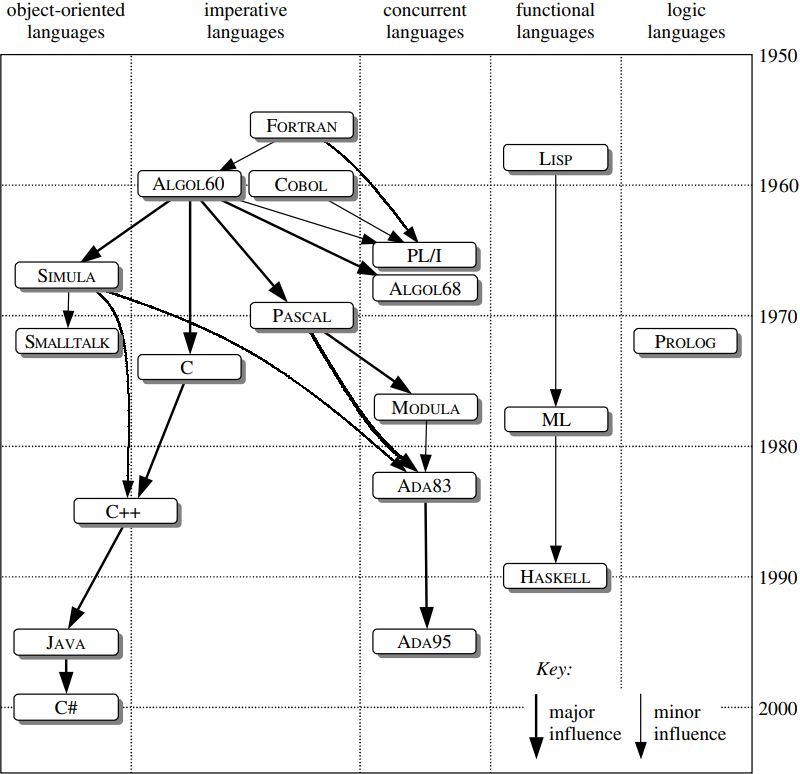
\includegraphics[width=\textwidth]{img/1.1-Programming-Languages.png}
    \caption{Dates and ancestry of major programming languages.}
    \label{fig:my_label}
\end{figure}

\textbf{Note:} \textit{This section can be read from book for further information.}




\end{document}
